\documentclass[11pt,a4paper]{article}
\usepackage{gtu-el-yazisi}
\begin{document}
\notbilgi{Nümerik Analiz}{1. Ders -- Kalkülüs Tekrarı}{Numerik-notlarim-1.ders.pdf}

\sayfa{1}
{\small\color{kursunkalem}Perşembe 10.12}

\section{Kalkülüs Tekrarı}
\noindent{\small\color{kursunkalem}\underline{süreklilik}}

\noindent
\begin{minipage}[c]{0.5\linewidth}
$\mathbb{R} = (-\infty, \infty)$ \ Reel Sayılar\\
$I \subset \mathbb{R}$ \ ``Aralık''\\
\hspace*{1em}$x_0 \in I$
\end{minipage}\hfill
\begin{minipage}[c]{0.45\linewidth}
\centering
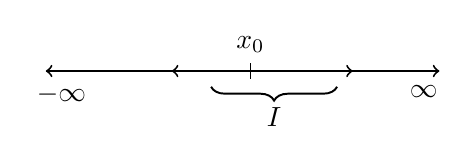
\begin{tikzpicture}[line width=0.7pt]
  \draw[<->] (0,0) -- (5,0);
  \node[below] at (0.2,-0.05) {$-\infty$};
  \node[below] at (4.8,-0.05) {$\infty$};
  \draw (2.6,0.1) -- (2.6,-0.1);
  \node[above] at (2.6,0.1) {$x_0$};
  \draw[<->] (1.6,0) -- (3.9,0);
  \draw[decorate, decoration={brace, amplitude=5pt, mirror}] (2.1,-0.2) -- (3.7,-0.2) node[midway, below=4pt] {$I$};
\end{tikzpicture}
\end{minipage}

\[
  \lim_{x\to x_0} f(x) = f(x_0) \qquad f(x)\ \text{fonksiyonu } x_0 \text{ noktasında süreklidir}
\]
$\forall x_0 \in I$ için sürekli ise $\rightarrow$ $I$'da sürekli\\
yani \ $f \in \underset{\substack{\downarrow\\ \text{continuous}}}{C}(I)$ \quad ; \ $C[a,b]$, \ $C(\mathbb{R})$

\[
  \lim_{x\to x_0} \frac{f(x) - f(x_0)}{x - x_0} \quad \text{varsa} \quad f(x)\text{'in türevi mevcuttur } x_0\text{'da.}
\]
\[
  \exists\ \lim \frac{f(x) - f(x_0)}{x - x_0} = f'(x_0) \;\rightarrow\; f\ \ x_0\text{'da sürekli}
\]
\hspace*{0.4\linewidth}türevlenebilir. \quad (tersi doğru değildir)

\medskip
\noindent $f \in C^{\textcircled{\scriptsize 1}}(I)$ \quad $\rightarrow$ birinci türev ile sürekli ise\\
{\scriptsize örnek}\quad $C^{n}(I)$ \quad $n$'ye kadar\\
\hspace*{3.2em}$C^{\infty}(I)$ \quad her mertebeden

\begin{ornek}
\noindent
\begin{minipage}[t]{0.55\linewidth}
\begin{align*}
  f(x) &= x^{3/2}\\
  f'(x) &= \frac{3}{2}\,x^{1/2}\\
  f''(x) &= \frac{3}{4}\,x^{-1/2}
\end{align*}
\end{minipage}\hfill
\begin{minipage}[t]{0.4\linewidth}
$x \in [0,1]$\\[4mm]
$f \in C^1(I)$\\[2mm]
$f \notin C^2(I)$
\end{minipage}
\end{ornek}

\sayfa{2}
\noindent
\begin{minipage}[c]{0.66\linewidth}
\begin{teorem}[1 (Rolle Teoremi)]
$f \in C[a,b]$ \qquad $f$ $(a,b)$ türevlenebilir.\\[1mm]
$f(a) = f(b) \;\rightarrow\; \underset{\text{en az bir}}{\exists}\ x = c$ {\small(``noktası'' üstü çizili)} $\in [a,b] \rightarrow f'(c) = 0$
\hfill{\small $f(b) = f(a)$}
\end{teorem}
\end{minipage}\hfill
\begin{minipage}[c]{0.3\linewidth}
\centering
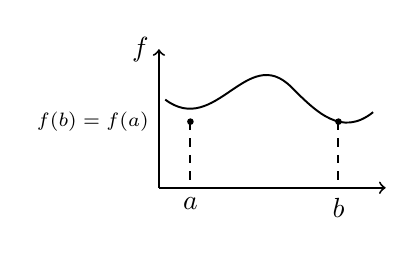
\begin{tikzpicture}[line width=0.7pt, scale=0.8]
  \draw[->] (0,0) -- (3.6,0);
  \draw[->] (0,0) -- (0,2.2) node[left] {$f$};
  \draw (0.1,1.4) .. controls (0.9,0.8) and (1.4,2.3) .. (2.1,1.6) .. controls (2.5,1.2) and (2.9,0.8) .. (3.4,1.2);
  \fill (0.5,1.05) circle (1.5pt) (2.85,1.05) circle (1.5pt);
  \draw[dashed] (0.5,1.05) -- (0.5,0) node[below] {$a$};
  \draw[dashed] (2.85,1.05) -- (2.85,0) node[below] {$b$};
  \node[left, font=\scriptsize] at (0,1.05) {$f(b) = f(a)$};
\end{tikzpicture}
\end{minipage}

\begin{ornek}
$f(x) = 1 - e^x + (e-1)\sin\left(\frac{1}{2}\,x\right)$\textsuperscript{*}'in en az bir noktada türevinin 0 olduğunu
gösteriniz. $[0,1]$ aralığında
\begin{align*}
  & f \in C^1[0,1]\\
  & f(0) = 0, \quad f(1) = 0 \qquad \checkmark\ \text{rolle teoremine göre türevi 0 olan bir nokta vardır}
\end{align*}
{\footnotesize\color{kursunkalem}* Claude notu: muhtemelen $\sin\left(\frac{\pi}{2}x\right)$ olmalı ($f(1) = 0$ ancak böyle sağlanır).\par}
\end{ornek}

\noindent
\begin{minipage}[c]{0.6\linewidth}
\begin{teorem}[2 (Ortalama Değer Teoremi)]
$f \in C[a,b]$ ve $f$ $(a,b)$ diferansiyellenebilir
\[
  c \in (a,b) \;\rightarrow\; f'(c) = \frac{f(b) - f(a)}{b - a}
\]
\end{teorem}
\end{minipage}\hfill
\begin{minipage}[c]{0.36\linewidth}
\centering
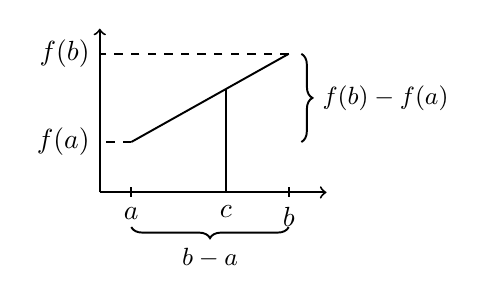
\begin{tikzpicture}[line width=0.7pt, scale=0.8]
  \draw[->] (0,0) -- (3.6,0);
  \draw[->] (0,0) -- (0,2.6);
  \draw (0.5,0.8) -- (3,2.2);
  \draw[dashed] (0.5,0.8) -- (0,0.8) node[left] {$f(a)$};
  \draw[dashed] (3,2.2) -- (0,2.2) node[left] {$f(b)$};
  \draw (0.5,0.08) -- (0.5,-0.08) node[below] {$a$};
  \draw (3,0.08) -- (3,-0.08) node[below] {$b$};
  \draw (2,0) -- (2,1.64);
  \node[below] at (2,-0.05) {$c$};
  \draw[decorate, decoration={brace, amplitude=4pt}] (3.2,2.2) -- (3.2,0.8) node[midway, right=4pt, font=\small] {$f(b) - f(a)$};
  \draw[decorate, decoration={brace, amplitude=4pt, mirror}] (0.5,-0.55) -- (3,-0.55) node[midway, below=4pt, font=\small] {$b - a$};
\end{tikzpicture}
\end{minipage}

\begin{teorem}[3 (Extremum değer Teoremi)]
{\small (Extremum: max ve min)}\\
\textcircled{\small 1}\ $f \in C[a,b]$ \qquad $c_1, c_2 \in [a,b]$ \ her $x \in [a,b]$
\[
  f(c_1) \le f(x) \le f(c_2)
\]
\textcircled{\small 2}\ $f$ $(a,b)$'de türevlenebilirse, $\rightarrow$ $c_1$ ve $c_2$ noktaları aralığın uç noktaları
yada $f'$'nin sıfır olduğu noktalar
\end{teorem}

\begin{ornek}[2]
$f(x) = \dfrac{2 - e^x + 2x}{3}$ \quad $I = [0,1]$ aralığında en büyük ve en küçük değerlerini bulunuz
\end{ornek}
\begin{cozum}
\begin{align*}
  f \in C^1[0,1] \;&\rightarrow\; f'(x) = \frac{-e^x + 2}{3}\\
  \text{kritik nokta} \Leftarrow f'(x) = 0 \;&\Rightarrow\; -e^x + 2 = 0\\
  e^x = 2 \;&\Rightarrow\; \boxed{x = \ln 2} \in [0,1]
\end{align*}
\[
  f(0) = \frac{2-1}{3} = \frac{1}{3} \underset{f_{\min}}{\underline{\simeq 0{,}\bar{3}}}, \qquad
  f(1) = \frac{4-e}{3} \simeq 0{,}43, \qquad
  f(\ln 2) = \frac{2\ln 2}{3} \underset{f_{\max}}{\underline{\simeq 0{,}46}}
\]
\end{cozum}

\sayfa{3}
\noindent
\begin{tikzpicture}[line width=0.7pt]
  \begin{axis}[width=5.2cm, height=3.4cm, xmin=0, xmax=1.15, ymin=0.25, ymax=0.5,
      axis lines=left, xtick=\empty, ytick={0.3333,0.43,0.46},
      yticklabels={$0{,}\bar{3}$, $0{,}43$, $0{,}46$}, tick label style={font=\scriptsize}]
    \addplot[domain=0:1, samples=40, smooth, murekkep] {(2-exp(x)+2*x)/3};
  \end{axis}
\end{tikzpicture}
\hspace{1em}{\small\color{kursunkalem}(Örnek 2'nin grafiği)}

\begin{teorem}[4 (Ara değer teoremi)]
$f \in C[a,b]$ \qquad $k$ \ $f(a)$ ile $f(b)$ arasında \okunamadi{keyfi} bir sayı o halde öyle $c \in (a,b)$
noktası bulunabilir ki: $f(c) = k$ olur. \quad $k = 0$
\end{teorem}

\sekilnotu[3]{Ara değer teoremi grafiği: $f(a)$ ve $k$ seviyelerinde yatay çizgiler; eğri $a$'da $f(a)$'nın
biraz üstünden başlıyor, aşağı inip yükseliyor, $c$'de $f(a)$ çizgisini kesiyor, tepe yapıp $b$'ye doğru
düşerken $k$ çizgisini kesiyor. Yatay eksende $a$, $c$, $b$ işaretli; $c$'den dikey çizgi.}

\noindent\underline{Sonuç:} \ Eğer $f \in C[a,b]$ \quad $f(a)\cdot f(b) < 0$\\
\hspace*{1em}o halde öyle bir $\underset{\text{(en az bir)}}{c} \in (a,b)$ bulunur ki $f(c) = 0$ olur.

\begin{ornek}[3]
$(x-2)^2 - \ln(x) = 0$ eşitliğinin $[1,2]$ aralığında en az bir kökünün olduğunu gösteriniz
\begin{align*}
  & f(1) = 1 > 0, \quad f(2) = -\ln 2 < 0 \qquad f(1)\cdot f(2) < 0\\
  & f(c) = 0
\end{align*}
\end{ornek}

\noindent Riemann manasında integrallenebilir \ $\Longleftarrow$ \ $f \in C[a,b]$
\[
  \int_a^b f(x)\,dx = \lim_{n\to\infty} \frac{b-a}{n}\sum_{i=1}^{n} f(x_i)
\]
\begin{center}
\begin{tikzpicture}[line width=0.6pt, scale=0.9]
  \draw[->] (-0.3,0) -- (5,0);
  \draw[->] (0,-0.3) -- (0,3.9);
  \foreach \i in {0,...,9}{
    \pgfmathsetmacro{\xl}{0.4+0.42*\i}
    \pgfmathsetmacro{\xr}{0.4+0.42*(\i+1)}
    \pgfmathsetmacro{\yy}{1.2+2.878*(\xr-0.4)-1.587*(\xr-0.4)^2+0.246*(\xr-0.4)^3}
    \draw[kursunkalem] (\xl,0) rectangle (\xr,\yy);
  }
  \draw[domain=0.4:4.6, samples=60, smooth] plot (\x, {1.2+2.878*(\x-0.4)-1.587*(\x-0.4)^2+0.246*(\x-0.4)^3});
  \node[below] at (0.4,0) {$a$};
  \node[below] at (4.6,0) {$b$};
  \node[below] at (1.9,-0.05) {$\frac{b-a}{n}$};
  \node[below] at (3.3,-0.05) {$f(x_i)$};
\end{tikzpicture}
\end{center}

\sayfa{4}
\begin{teorem}[5 (İntegral için ara değer teoremi)]
$f \in C[a,b]$ ve $g$ $[a,b]$ aralığında R.A.İ ve işaret değiştirmez
\[
  c \in (a,b) \qquad \int_a^b f(x)\,g(x)\,dx = f(c)\int_a^b g(x)\,dx
\]
\end{teorem}
\noindent\underline{\small Sonuç}\qquad $g(x) = 1 \;\rightarrow\; f(c) = \dfrac{1}{b-a}\displaystyle\int_a^b f(x)\,dx$

\subsection{Taylor polinom ve Serisi}
\begin{teorem}[(Taylor)]
$f \in C^n[a,b]$, $f^{(n+1)}$ türevi $[a,b]$ aralığında mevcut (süreklilik şart değil) $x_0 \in [a,b]$.
Bu durumda, her $x \in [a,b]$ için, $x_0$ ve $x$ noktaları arasından
\[
  \xi = \xi(x) \quad \text{bulunabilir ki}
\]
\[
  \underset{\text{\scriptsize verilen fonk.}}{f(x)} = \underset{\text{\scriptsize tahmini değer}}{P_n(x)}
  + \underset{\text{\scriptsize kesim hatası}}{R_n(x)}
  \;\nearrow\; R_n(x) = \frac{f^{(n+1)}(\xi)}{(n+1)!}(x-x_0)^{n+1}
\]
\end{teorem}
{\small n'inci dereceden taylor polinomu}
\begin{align*}
  P_n(x) &= f(x_0) + \frac{f'(x_0)}{1!}(x-x_0) + \frac{f''}{2!}(x-x_0)^2 + \cdots + \frac{f^{(n)}}{n!}(x-x_0)^n\\
  &= \sum_{k=0}^{n} \frac{f^{(k)}(x_0)}{k!}(x-x_0)^k
\end{align*}
$n \to \infty$ \quad $P_n(x)$ limitte Taylor serisini verir
\[
  f(x) = \sum_{k=0}^{\infty} \frac{f^{(k)}(x_0)}{k!}(x-x_0)^k
\]
\hspace*{2em}$x_0 = 0$ \quad Mclaurin Serisi

\begin{ornek}[4]
$f(x) = (1+x)^{1/2}$ fonk için \hfill
\begin{tabular}[t]{l}
a) 3. mertebeden T.P\\
b) $P_3(x) \rightarrow f(\sqrt{1{,}1})$'i tahmin\\
c) Tahminin hatasını değerlendir
\end{tabular}
\end{ornek}
\begin{align*}
  f(x) &= P_3(x) + R_3(x)\\
  P_3(x) &= f(0) + f'(0)\,x + \frac{f''(0)}{2!}\,x^2 + \frac{f'''(0)}{3!}\,x^3\\
  R_3(x) &= \frac{f^{(4)}(\xi)}{4!}\,x^4 \qquad \xi \in (0,x) \ \text{veya}\ \xi \in (x,0)
\end{align*}
\begin{align*}
  f(x) &= (1+x)^{1/2} &&\Rightarrow f(0) = 1\\
  f'(x) &= \frac{1}{2}(1 + x^{1/2})^{-1/2}\footnotemark &&\Rightarrow f'(0) = \frac{1}{2}\\
  f''(x) &= -\frac{1}{4}(1+x)^{-3/2} &&\Rightarrow f''(0) = -\frac{1}{4}\\
  f'''(x) &= \frac{3}{8}(1+x)^{-5/2} &&\Rightarrow f'''(0) = \frac{3}{8}
\end{align*}
\footnotetext{Claude notu: muhtemelen $\frac{1}{2}(1+x)^{-1/2}$ olmalı.}

\sayfa{5}
\hfill $\xi \in (0,x)$ veya $\xi \in (x,0)$
\[
  f^{(4)}(x) = -\frac{15}{16}(1+x)^{-7/2} \;\Rightarrow\; f^{(4)}(\xi) = -\frac{15}{16}(1+\xi)^{-7/2}
\]
o zaman
\begin{align*}
  P_3(x) &= 1 + \frac{1}{2}\,x - \frac{1}{8}\,x^2 + \frac{1}{16}\,x^3\\
  R_3(x) &= -\frac{5}{128}(1+\xi)^{-7/2}\,x^4
\end{align*}
$f = \sqrt{1{,}1} \;\Rightarrow\; x = 0{,}1$
\begin{align*}
  P_3 &= 1 + \frac{1}{2}(0{,}1) - \frac{1}{8}(0{,}1)^2 + \frac{1}{16}(0{,}1)^3\\
      &= 1 + \frac{1}{20} - \frac{1}{800} + \frac{1}{16000} \cong 1{,}0488125
\end{align*}
\begin{align*}
  R_3(0{,}1) &= -\frac{5}{128}\cdot\frac{1}{(1+\xi)^{7/2}}\cdot\frac{1}{10000}\\
  |R_3| &= |f(0{,}1) - P_3|
\end{align*}
\[
  R_3(0{,}1) = -\frac{5}{128}\cdot\frac{1}{(1+\boxed{\xi})^{7/2}}\cdot\frac{1}{10000} \le
\]
\hspace*{0.3\linewidth}{\small $\swarrow$ 0 veriyoruz en büyük hatayı bulmak için}
\[
  \simeq 3{,}91\cdot10^{-6}
\]
\begin{gather*}
  P_3(0{,}1) - 3{,}91\cdot10^{-6} \le f(0{,}1) \le P_3(0{,}1) + 3{,}91\cdot10^{-6}\\
  1{,}04880859 \le \underset{\substack{\shortparallel\\ 1{,}0488088}}{\sqrt{1{,}1}} \le 1{,}0488164
\end{gather*}

\begin{ornek}[5]
$f(x) = (1+x)^{1/2}$ \quad $x_0 = 0$ noktasında $P_3$ ile
\[
  \int_0^{0{,}1} (1+x)^{1/2}\,dx
\]
\end{ornek}

\sayfa{6}
\begin{align*}
  P_3(x) &= 1 + \frac{1}{2}\,x - \frac{1}{8}\,x^2 + \frac{1}{16}\,x^3\\
  \int_0^{0{,}1} P_3(x)\,dx &= \int_0^{0{,}1}\left(1 + \frac{1}{2}\,x - \frac{1}{8}\,x^2 + \frac{1}{16}\,x^3\right)dx\\
  &= \left[x + \frac{x^2}{4} - \frac{x^3}{24} + \frac{x^4}{64}\right]_{x=0}^{x=0{,}1} \simeq 0{,}1025\\
  \int_0^{0{,}1} R_3(x)\,dx &= \int_0^{0{,}1} -\frac{5}{128}(1+\xi)^{-7/2}\,x^4
     \le \int_0^{0{,}1}\left(-\frac{5}{128}\,x^4\right)dx\\
  &= -\frac{1}{128}\,x^5\bigg]_0^{0{,}1} =
\end{align*}

\begin{ornek}
$f(x) = e^x\cos x$ fonksiyonu için\\
a) $x_0 = 0$ noktasında 2. mertebeden $P_2(x)$ Taylor polinomunu hesaplayınız\\
b) $P_2(0{,}5)$'i kullanarak $f(0{,}5)$ değerini tahmini hesaplayınız ve hatasını değerlendiriniz\\
c) $|f(x) - P_2(x)|$ hatasını $[0,1]$ aralığında değerlendiriniz \hfill{\small(solda yuvarlak içinde: ``ödev'')}\\
d) $\displaystyle\int_0^1 P_2(x)\,dx$'i kullanarak $\displaystyle\int_0^1 f(x)\,dx$ integralinin değerini tahmini
hesaplayınız ve hatasını değerlendiriniz
\end{ornek}

\noindent a)
\[
  f(x) = \underset{\substack{\text{2. mertebeden}\\ \text{Taylor polinomu}\\ \text{(tahmini değer)}}}{\underbrace{P_2(x)}}
  + \underset{\substack{\text{kalan terim}\\ \text{(kesim hatası)}}}{\underbrace{R_2(x)}}
\]
\[
  f(x) = \sum_{k=0}^{\infty} \frac{f^{(k)}(x_0)}{k!}(x-x_0)^k \;; \quad x_0 = 0 \text{ için yeniden yazalım}
\]
\[
  f(x) = \sum_{k=0}^{\infty} \frac{f^{(k)}(x_0)}{k!}\,(x)^k
\]
$\Rightarrow$ Bu durumda $P_2(x)$
\begin{align*}
  P_2(x) &= \sum_{k=0}^{2} \frac{f^{(k)}(0)}{k!}\,x^k = f(0) + \frac{f'(0)}{1!}\footnotemark + \frac{f''(0)}{2!}\,x^2\\
  R_2(x) &= \frac{f'''(\xi)}{3!}\,x^3 \qquad \xi \in (0,x) \ \text{veya}\ \xi \in (x,0)
\end{align*}
\footnotetext{Claude notu: muhtemelen $\frac{f'(0)}{1!}\,x$ olmalı.}

\sayfa{7}
\noindent Türevleri hesaplayalım
\begin{align*}
  f(x) &= e^x\cos x \;\Rightarrow\; f(0) = 1\\
  f'(x) &= e^x\cos x + (-\sin x)\,e^x = e^x(\cos x - \sin x) \;\Rightarrow\; f'(0) = 1\\
  f''(x) &= e^x(\cos x - \sin x) + (-\sin x - \cos x)\,e^x =\\
         &= -2e^x\sin x\\
  f''(0) &= 0
\end{align*}
\begin{align*}
  f'''(x) &= -2\left[e^x\sin x + \cos x\,e^x\right] = -2e^x(\sin x + \cos x)\\
  f'''(\xi) &= -2e^{\xi}(\sin\xi + \cos\xi)
\end{align*}
\begin{align*}
  P_2(x) &= 1 + x\\
  R_2(x) &= -\frac{1}{3}\,e^{\xi}(\sin\xi + \cos\xi)\,x^3\\
  P_2(0{,}5) &= 1{,}5
\end{align*}
\[
  R(0{,}5)\footnotemark = P_2(0{,}5) + \underbrace{R_2(0{,}5)}_{\text{hata terimi}}
\]
\footnotetext{Claude notu: muhtemelen $f(0{,}5)$ olmalı.}
\begin{align*}
  R_2(0{,}5) &= -\frac{1}{3}\,e^{\xi}(\sin\xi + \cos)\,(0{,}5)^3\\
             &= -\frac{1}{3}\,e^{\xi}(\sin\xi + \cos)\,\frac{1}{8}\\
             &= -\frac{1}{24}\,e^{\xi}(\sin\xi + \cos\xi)
\end{align*}
\[
  \xi \in [0;\ 0{,}5]
\]
\begin{center}
$0{,}5$'te max değer alır
\end{center}
\[
  |R_2(0{,}5)| \le \frac{1}{24}\,e^{\xi}(\sin\xi + \cos\xi) \le 0{,}09322200499
\]
\[
  \underset{\substack{\text{gerçek değer}\\ 1{,}44688903658}}{\underline{f(0{,}5)}}
  - \underset{\substack{\text{tahmini değer}\\ 1{,}5}}{\underline{P_2(0{,}5)}} = R_2(0{,}5)
\]
\begin{gather*}
  R_2(0{,}5)\footnotemark - 0{,}09322200499 \le f(0{,}5) \le\\
  P_2(0{,}5) + 0{,}09322200499
\end{gather*}
\footnotetext{Claude notu: muhtemelen $P_2(0{,}5)$ olmalı.}

\end{document}
